\chapter{Literature Review}
This chapter provides an overview of forecasting methods relevant to the research for offshore wind turbine installations. Chapter \ref{lit:overview} explores three conventional techniques—Numerical Weather Prediction (NWP), Statistical Forecasting (SF), and Ensemble Forecasting (EF)—which have been widely adopted in meteorological and offshore applications. Their respective strengths and limitations are presented to highlight why more advanced solutions may be necessary. Next, Chapters \ref{lit:hybrid_models}, \ref{lit:probabilistic_model}, \ref{lit:LSTM_literature} examine hybrid ARIMA–ANN models, Bayesian Neural Networks (BNNs), and LSTM-based deep learning approaches. They are each designed to address shortcomings in standard forecasting practice. In Chapter \ref{lit:comparative} the three models are compared to each other. Finally, Chapter \ref{lit:previous} reviews two prior studies \cite{boer2022installation, overvliet2023uncertainty} that offer practical insights into the performance of these models under real-world conditions and underscore the importance of accurate met-ocean predictions.

\section{Overview of Current Weather Forecasting Techniques}
\label{lit:overview}
Accurate weather forecasting is important in offshore wind turbine installations. Where significant wave height, wind speed, and wave frequency directly affect operational windows for installing offshore wind turbines. Current forecasting methods are Numerical Weather Prediction (NWP), Statistical Forecasting (SF), and Ensemble Forecasting (EF). While several other forecasting techniques are available, this research focuses on NWP, SF, and EF, given that these particular methods have been validated substantially in both meteorological and offshore applications. They are showing skill in simulating multiple physical processes, identifying many historical trends, and quantifying uncertainty (\cite{box2015time, leutbecher2008ensemble}). These techniques relate to the research because NWP offers a physical basis for understanding atmospheric dynamics. Secondly, SF gives a computationally efficient way to model past patterns. Finally, EF improves forecast reliability by incorporating uncertainty, all of which have complementary strengths. These techniques together provide a framework for this research, in the development of forecasting models.

\subsection{Numerical Weather Prediction (NWP)}
Numerical Weather Prediction was initially developed to model atmospheric behaviour. It can also be used in offshore contexts. NWP models solve physical equations using input from met-ocean data, such as wave height, sea surface temperature, ocean currents, and wind. This data is typically gathered from buoys, ships, or satellites, although ensuring complete numerical coverage can be challenging, especially for phenomena like wind shears or sudden squalls.

\paragraph{Principles of NWP}
NWP relies on several physical equations:
\begin{itemize}
    \item \textbf{Navier-Stokes Equations}: Govern fluid motion.
    \item \textbf{Continuity Equation}: Ensures mass conservation.
    \item \textbf{Thermodynamic Energy Equation}: Accounts for heat exchanges between atmosphere and ocean.
\end{itemize}
These equations are linked via the Equation of State, which relates pressure, density, and temperature, allowing for forecasts ranging from several hours to days (\cite{coiffier2011, bauer2015}).\\

\noindent\textbf{Strengths of NWP Models}

\noindent Because NWP is rooted in the fundamental physics of air–water interactions, it can achieve accuracy under many conditions. Their ability to assimilate real-time data allows them to capture fast changes effectively (\cite{coiffier2011}).\\

\noindent\textbf{Limitations in Offshore Applications}

\noindent On the other hand, NWP models are computationally intensive, requiring significant resources \cite{bauer2015}. They typically operate at a big spatial resolution, which may not capture the localized conditions essential for offshore wind installations. Additionally, despite continuous improvements—adding roughly one extra day of forecast accuracy per decade—the forecast horizon often remains too short for some operational requirements.

\subsection{Statistical Forecasting (SF)}
\label{statistical_forecasting}
Statistical Forecasting (SF) methods analyse historical data to identify trends, seasonality, and correlations, assuming that past patterns can predict future conditions. Unlike NWP, which is based on fundamental physics, SF approaches rely on linear (or in some cases slightly non-linear) relationships extracted from the time series.

\paragraph{ARIMA Models}
Auto-Regressive Integrated Moving Average (ARIMA) models decompose time-series data into autoregressive (AR) and moving average (MA) components, handling both stationary and non-stationary data. The general ARIMA framework is typically expressed as:
\begin{equation}
    \varphi(B) \, z_t = \Phi(B) \, \nabla^d z_t = \theta_0 + \theta(B) \, a_t,
    \label{eq:general_arima}
\end{equation}
where $B$ is the backshift operator, and $\nabla^d$ denotes differencing $d$ times. These models are efficient for detecting consistent trends but may struggle with abrupt or extreme changes \cite{box2015time}.

\paragraph{Exponential Smoothing (Holt--Winters)}
Exponential Smoothing assigns exponentially decreasing weights to older observations, allowing recent data to have a stronger influence on forecasts. Holt-Winters (triple exponential smoothing) is especially relevant for weather data with both trend and seasonality:
\begin{equation}
    \hat{y}_{t+h} = (L_t + h T_t) \, S_{t+h - m(k+1)},
    \label{eq:forecast_holt_winters}
\end{equation}
where $L_t$ is the level, $T_t$ the trend, and $S_t$ the seasonal component (\cite{hyndman2018forecasting}).\\

\noindent\textbf{Strengths of SF Models}

\noindent SF models are computationally efficient, enabling fast execution compared to high-dimensional physical models. They are also highly adaptable, allowing for easy updates as new data become available, which makes them particularly effective for short-term forecasts.\\

\noindent\textbf{Limitations in Offshore Applications}

\noindent Yet, SF models usually lean on linear assumptions, making them less effective at handling sharp fluctuations or unusual conditions. Additionally, their heavy reliance on historical patterns poses challenges for long-term forecasting in dynamic offshore environments (\cite{Zhang2019}). These limitations can be overcome with a hybrid model, discussed in Chapter \ref{lit:hybrid_models}.

\newpage
\subsection{Ensemble Forecasting (EF)}
\label{ensemble_forecasting}
Ensemble Forecasting (EF) generates a set of forecasts by introducing small variations in initial conditions or model parameters. This will lead to a set of outcomes known as ensemble members. Even small uncertainties in the initial state can lead to significantly divergent forecasts, particularly under chaotic weather situations (\cite{leutbecher2008ensemble}). By sampling a range of possible initial conditions, EF captures a spectrum of possible future states. Consequently, it provides a probabilistic rather than a single deterministic forecast. This probabilistic framework is particularly valuable in weather forecasting, as it enables forecasters and decision-makers to assess the likelihood of various outcomes and manage risks more effectively (\cite{gneiting2005weather}).\\

\noindent\textbf{Strengths of EF Models}

\noindent EF models provide valuable uncertainty quantification by offering probabilities for different scenarios, which aids in risk management for offshore projects. They tend to achieve higher accuracy on average by averaging multiple ensemble members, and their adaptability allows new observations to be constructed in real-time, refining the forecasts.\\

\noindent\textbf{Limitations of EF Models}

\noindent However, running multiple simulations makes EF models computationally expensive, potentially exceeding real-time constraints. Additionally, managing and interpreting the spread of outcomes can be challenging, especially when dealing with extreme weather events. These extreme events will directly impact the windows of operation. 

\subsection{Summary of Current Forecasting Techniques}
To provide an overview, Table~\ref{tab:forecasting_summary} summarizes the primary strengths and limitations of each forecasting technique in offshore applications.

\begin{table}[h!]
\centering
\caption{Comparative summary of current forecasting techniques for offshore applications}
\label{tab:forecasting_summary}
\begin{tabular}{|p{2cm}|p{6.3cm}|p{6cm}|}
\hline
\centering \textbf{Technique} & \textbf{Strengths} & \textbf{Limitations} 
\\ \hline 
\vspace{5pt}
\centering\textbf{NWP} & 
Based on physical laws\newline
Capturing large-scale dynamics\newline
Real-time data adaptation
& 
High computational cost\newline
Big spatial resolution\newline
Limited forecast horizon
\\ \hline
\vspace{5pt}
\centering\textbf{SF} &
Low computational cost\newline
Effective in capturing trends/seasonality\newline
Easy to update with new data
&
Primarily linear assumptions\newline
Less effective for extreme events\newline
Reliance on historical patterns
\\ \hline
\vspace{5pt}
\centering\textbf{EF} &
Accounts for uncertainties\newline
Provides probabilistic forecasts\newline
Can improve average accuracy
&
High computational cost\newline
Complex to implement\newline
Interpretation challenges
\\ \hline
\end{tabular}
\end{table}

\noindent Based on Table \ref{tab:forecasting_summary}, it is evident that no single forecasting technique is ideally suited to meet the unique operational requirements of a specific offshore site. However, they give valuable insight into how the models are constructed and how the models could be enhanced. Where the SF model techniques are constructed to capture linear behaviour, they often miss non-linear components. This shortcoming motivates the development of a Hybrid Model, Chapter \ref{lit:hybrid_models}. Similarly, EF models offer robust uncertainty quantification but have high computational time and interpretation challenges. These can be removed in a new probabilistic model, Chapter \ref{lit:probabilistic_model}. Which will lower computational time by making use of dropout ratios. Finally, to capture complex dependencies in the dynamic weather, the model in Chapter \ref{lit:LSTM_literature} is further investigated. In summary, these advanced models were specifically designed to overcome the limitations of NWP, SF, and EF. Together, they form an approach that underpins the forecasting techniques developed in this research.
\newpage
\section{Hybrid Models, ARIMA and ANN}
\label{lit:hybrid_models}
Where the ARIMA model mentioned in chapter \ref{statistical_forecasting} finds linearity in past data, it is unable to capture non-linear changes (\cite{zhang2003time}). That is where the artificial neural network (ANN) comes in, it will find non-linear cases based on the residuals of the ARIMA model. ANNs are inspired by the human brain, and with different interconnected nodes, it becomes possible to identify patterns by learning from examples. The ANN network, visualized in Figure \ref{fig:hybrid_ann_diagram}, is constructed in three different layers, the input layer, one or more hidden layers, and an output layer. Each connection between layers is assigned a weight that is iteratively optimized during training to reduce the discrepancy between the network's predictions and the actual outputs. (\cite{haykin1994neural, buyuksahin2019improving}).

\begin{figure}[ht]
    \centering
    \begin{tikzpicture}[x=1.8cm, y=1.2cm, >=stealth]
        \node[circle, draw, fill=green!20, minimum size=1cm] (A) {ARIMA};
        \node[above=1.36cm of A] {ARIMA Model};
        
        \node[circle, draw, fill=blue!20, minimum size=1cm] (I) [right of=A, xshift=2cm] {Residual};
        \node[above=1.18cm of I] {Input};
        
        \node[circle, draw, fill=blue!20, minimum size=1cm] (H11) [right of=I, xshift=2cm, yshift=1.5cm] {H1};
        \node[circle, draw, fill=blue!20, minimum size=1cm] (H12) [right of=I, xshift=2cm] {H1};
        \node[circle, draw, fill=blue!20, minimum size=1cm] (H13) [right of=I, xshift=2cm, yshift=-1.5cm] {H1};
        \node[above=1.5cm of H12] {Hidden Layer 1};
        
        \node[circle, draw, fill=blue!20, minimum size=1cm] (H21) [right of=H11, xshift=2cm, yshift=-0.6cm] {H2};
        \node[circle, draw, fill=blue!20, minimum size=1cm] (H22) [right of=H13, xshift=2cm, yshift=0.6cm] {H2};
        \node[above=0.59cm of H21] {Hidden Layer 2};
        
        \node[circle, draw, fill=blue!20, minimum size=1cm] (O) [right of=H12, xshift=4.5cm] {Output};
        \node[above=1.3cm of O] {Output};
        
        \draw[->, thick] (A) -- node[above, sloped] {} (I);
        
        \draw[->, thick] (I) -- node[above, sloped] {$w$} (H11);
        \draw[->, thick] (I) -- node[above, sloped] {$w$} (H12);
        \draw[->, thick] (I) -- node[above, sloped] {$w$} (H13);
        
        \draw[->, thick] (H11) -- node[above, sloped] {$w$} (H21);
        \draw[->, thick] (H12) -- node[above, sloped] {$w$} (H21);
        \draw[->, thick] (H12) -- node[above, sloped] {$w$} (H22);
        \draw[->, thick] (H13) -- node[above, sloped] {$w$} (H22);
        
        \draw[->, thick] (H21) -- node[above, sloped] {$w$} (O);
        \draw[->, thick] (H22) -- node[above, sloped] {$w$} (O);

    \end{tikzpicture}
    \caption{Visualization of a Hybrid ARIMA–ANN Model. The ARIMA model generates a forecast, and its residual is used as the input to a feedforward neural network consisting of two hidden layers and one output layer.}
    \label{fig:hybrid_ann_diagram}
\end{figure}

\noindent From the book \cite{haykin1994neural}, several ANN formulas are used in the application of weather forecasting from time series. Firstly, the ANN formula can be simplified to a feed-forward neural network FFNN, in which the data flows from the input to the output without looping back. The basic Formula \ref{eq:ffnn_structure} for each node/neuron.

\begin{equation}
    y = f\left(\sum_{i=1}^n w_i x_i + b\right)
    \label{eq:ffnn_structure}
\end{equation}

\noindent The activation Formula \ref{eq:sigmoid_activation} and Formula \ref{eq:relu_activation} which can both be relevant in weather application. Where Formula \ref{eq:sigmoid_activation} is mostly useful in probabilistic output and Formula \ref{eq:relu_activation} is effective for hidden layers in the data, so there is no vanishing of the gradient (\cite{haykin1994neural}).

\begin{equation}
    f(x) = \frac{1}{1 + e^{-x}}
    \label{eq:sigmoid_activation}
\end{equation}

\begin{equation}
    f(x) = \max(0, x)
    \label{eq:relu_activation}
\end{equation}

\noindent For the training of the ANN, a back-propagation is used with the weighted values between neuron i and j, this is done with Formula \ref{eq:backpropagation_update}
\begin{equation}
    \Delta w_{ij} = -\eta \frac{\partial E}{\partial w_{ij}}
    \label{eq:backpropagation_update}
\end{equation}

\noindent The mean squared error, Formula \ref{eq:mse_loss}, can be used to minimize the error, and so finding better-weighted values
\begin{equation}
    E = \frac{1}{N} \sum_{i=1}^{N} (y_i - \hat{y}_i)^2
    \label{eq:mse_loss}
\end{equation}

\noindent To avoid over-fitting of the data, regularization, such as weight decay, can be used, shown in Formula \ref{eq:l2_regularization}.  
\begin{equation}
    E = \frac{1}{N} \sum_{i=1}^{N} (y_i - \hat{y}_i)^2 + \lambda \sum_{j=1}^{M} w_j^2
    \label{eq:l2_regularization}
\end{equation}

\noindent Using Formula \ref{eq:general_arima} for the linear patterns in the data and finding the residual error with Formula \ref{eq:residual_error}, this will capture the non-linear part of the forecast. 

\begin{equation}
    e(t) = y(t) - y_{\text{ARIMA}}(t)
    \label{eq:residual_error}
\end{equation}

\noindent Applying this $e(t)$ in the ANN formula as input data, the model can be trained to model this non-linear behaviour. This will eventually result in the forecasted non-linear component $y_{ANN}$ which is equal to the $y$ in Formula \ref{eq:ffnn_structure}. Using one of the activation functions \ref{eq:sigmoid_activation} \ref{eq:relu_activation} the ANN can be trained and adapted to find a non-linear solution. Combining the ARIMA model and the ANN model is done with Formula \ref{eq:hybrid_forecast}, the mean squared error, Formula \ref{eq:hybrid_mse}, is then used to further find the weights for the ANN model.

\begin{equation}
    y_{\text{hybrid}}(t) = y_{\text{ARIMA}}(t) + y_{\text{ANN}}(t)
    \label{eq:hybrid_forecast}
\end{equation}

\begin{equation}
    E = \frac{1}{N} \sum_{i=1}^{N} \left(y_i - y_{\text{hybrid}, i}\right)^2
    \label{eq:hybrid_mse}
\end{equation}

\noindent By merging ARIMA and ANN elements, the hybrid approach incorporates linear and non-linear dynamics in the final forecast (\cite{zhang2003time}). This combination makes it more suitable for the implementation of complex and rapid changes in offshore forecasting.

\section{Probabilistic Models, BNN}
\label{lit:probabilistic_model}
The Bayesian Neural Network, BNN, is a class of neural networks that incorporates uncertainties by learning a distribution between the different inputs. It can be seen as a type of neural network, but with an extra step in which it incorporates probabilistic reasoning. For this model to work, the conditional probability of each connection is found. This will allow the model to capture the uncertainty in how each weight influences the output. To achieve this, the model can be trained with the inputted data. A learning algorithm is used, which can be divided into two steps, firstly, a quality measure will measure the quality of the estimated parameters. Secondly, a search algorithm to find the BNN with the highest quality (\cite{cofino2002bayesian}). BNNs rely on Bayes’ theorem Formula \ref{eq:bayes_theorem}, which updates the prior probability distribution of each weight based on observed data, yielding a posterior distribution.  

\begin{equation}
    p(w|D) = \frac{p(D|w) \, p(w)}{p(D)}
    \label{eq:bayes_theorem}
\end{equation}

\noindent To make probabilistic predictions, BNNs integrate overall weight values. This results in a prediction distribution for an output $\hat{y}$, instead of giving a single output. The Formula \ref{eq:bayesian_prediction} integrates over the posterior distribution, $P(w|D)$. The model averages the likelihood of $\hat{y}$ over all possible weight configurations. With the usage of this model, the output can be found and the error concerning the actual values can be kept to a minimum. The result is that BNN will produce a predictive distribution of the outcome (\cite{mackay1992bayesian}).

\begin{equation}
    p(\hat{y}|D) = \int p(\hat{y}|w) \, p(w|D) \, dw
    \label{eq:bayesian_prediction}
\end{equation}

\noindent The computational time will be too long if the BNN is done in this way, while there are too many different variables. All interconnections between these variables will have different weights which need to be found. To reduce this time, Monte Carlo Dropout, MCD, will be used. MCD  will approximate the integration during the prediction phase, Formula \ref{eq:bayesian_prediction}. So, instead of using a fully Bayesian approach as visualized in Figure \ref{fig:mcd_vs_standard}a, random nodes, in the hidden layers, between one another will be dropped, this is repeated multiple times to produce a stochastic set of outputs. The final prediction follows from averaging the outputs of these multiple stochastic sets, this is visualized in Figure \ref{fig:mcd_vs_standard}b. This will decrease computational time significantly and with multiple simulations, the error from the drop-outs can be made insignificant (\cite{mae2022uncertainty,gal2016dropout}).

\begin{figure}[ht]
    \centering
    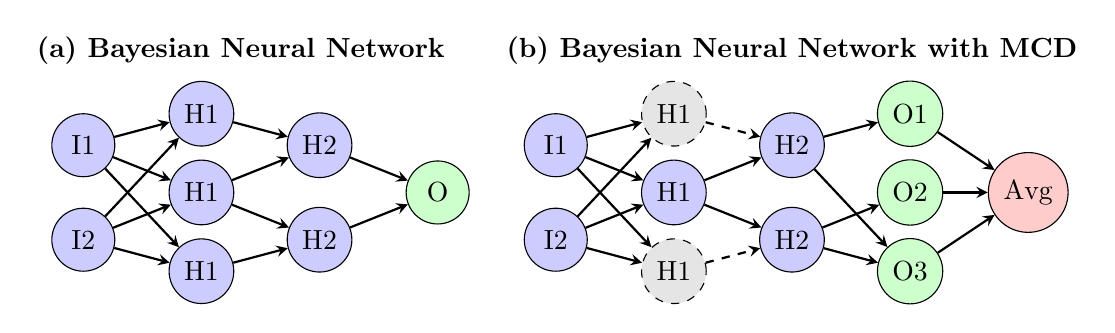
\begin{tikzpicture}[x=1.0cm, y=0.8cm, >=stealth]

        % === Standard Neural Network (Without MCD) ===
        \node[draw=none] at (2, 3) {\textbf{(a) Bayesian Neural Network}};

        % Input Layer (Left Side)
        \node[circle, draw, fill=blue!20, minimum size=0.8cm] (I1) at (0, 1.5) {I1};
        \node[circle, draw, fill=blue!20, minimum size=0.8cm] (I2) at (0, 0) {I2};

        % Hidden Layer 1 (No Dropout)
        \node[circle, draw, fill=blue!20, minimum size=0.8cm] (H11) at (1.5, 2) {H1};
        \node[circle, draw, fill=blue!20, minimum size=0.8cm] (H12) at (1.5, 0.75) {H1};
        \node[circle, draw, fill=blue!20, minimum size=0.8cm] (H13) at (1.5, -0.5) {H1};

        % Hidden Layer 2
        \node[circle, draw, fill=blue!20, minimum size=0.8cm] (H21) at (3, 1.5) {H2};
        \node[circle, draw, fill=blue!20, minimum size=0.8cm] (H22) at (3, 0) {H2};

        % Output Layer (Standard NN)
        \node[circle, draw, fill=green!20, minimum size=0.8cm] (O1) at (4.5, 0.75) {O};

        % Connections (Standard NN)
        \draw[->, thick] (I1) -- (H11);
        \draw[->, thick] (I1) -- (H12);
        \draw[->, thick] (I1) -- (H13);
        \draw[->, thick] (I2) -- (H11);
        \draw[->, thick] (I2) -- (H12);
        \draw[->, thick] (I2) -- (H13);

        \draw[->, thick] (H11) -- (H21);
        \draw[->, thick] (H12) -- (H21);
        \draw[->, thick] (H12) -- (H22);
        \draw[->, thick] (H13) -- (H22);

        \draw[->, thick] (H21) -- (O1);
        \draw[->, thick] (H22) -- (O1);

        \node[draw=none] at (9, 3) {\textbf{(b) Bayesian Neural Network with MCD}};

        \node[circle, draw, fill=blue!20, minimum size=0.8cm] (I1b) at (6, 1.5) {I1};
        \node[circle, draw, fill=blue!20, minimum size=0.8cm] (I2b) at (6, 0) {I2};
        
        \node[circle, draw, fill=gray!20, dashed, minimum size=0.8cm] (D1) at (7.5, 2) {H1};
        \node[circle, draw, fill=blue!20, minimum size=0.8cm] (D2) at (7.5, 0.75) {H1};
        \node[circle, draw, fill=gray!20, dashed, minimum size=0.8cm] (D3) at (7.5, -0.5) {H1};

        \node[circle, draw, fill=blue!20, minimum size=0.8cm] (H21b) at (9, 1.5) {H2};
        \node[circle, draw, fill=blue!20, minimum size=0.8cm] (H22b) at (9, 0) {H2};

        \node[circle, draw, fill=green!20, minimum size=0.8cm] (O1b) at (10.5, 2) {O1};
        \node[circle, draw, fill=green!20, minimum size=0.8cm] (O2b) at (10.5, 0.75) {O2};
        \node[circle, draw, fill=green!20, minimum size=0.8cm] (O3b) at (10.5, -0.5) {O3};

        \node[circle, draw, fill=red!20, minimum size=0.8cm] (Final) at (12, 0.75) {Avg};

        \draw[->, thick] (I1b) -- (D1);
        \draw[->, thick] (I1b) -- (D2);
        \draw[->, thick] (I1b) -- (D3);
        \draw[->, thick] (I2b) -- (D1);
        \draw[->, thick] (I2b) -- (D2);
        \draw[->, thick] (I2b) -- (D3);

        \draw[->, thick, dashed] (D1) -- (H21b);
        \draw[->, thick] (D2) -- (H21b);
        \draw[->, thick] (D2) -- (H22b);
        \draw[->, thick, dashed] (D3) -- (H22b);

        \draw[->, thick] (H21b) -- (O1b);
        \draw[->, thick] (H22b) -- (O2b);
        \draw[->, thick] (H21b) -- (O3b);
        \draw[->, thick] (H22b) -- (O3b);

        \draw[->, thick] (O1b) -- (Final);
        \draw[->, thick] (O2b) -- (Final);
        \draw[->, thick] (O3b) -- (Final);

    \end{tikzpicture}
    \caption{(a) Standard Neural Network: A traditional feed-forward structure with fixed weights. 
    (b) Neural Network with Monte Carlo Dropout (MCD): Dropout is applied during inference, producing different outputs across multiple forward passes, averaging to approximate Bayesian inference.}
    \label{fig:mcd_vs_standard}
\end{figure}

\noindent BNNs that employ Monte Carlo Dropout can efficiently produce both forecasts and uncertainty estimates. By using the expected forecast and uncertainty estimation, it is well usable in offshore weather forecasting. 

\section{Deep Learning Models, LSTM}
\label{lit:LSTM_literature}
Deep learning models can capture complex non-linear behaviour in time series forecasting. Given the large fluctuations in weather patterns over time and across regions, LSTMs offer a promising solution for improving forecast accuracy. A deep learning model, which is used in other forecasting applications, and on a smaller scale on weather, is long-short term memory, LSTM. The reason for usage is that it can capture both short-term fluctuations and long-term dependencies (\cite{siami2019comparison}). The model can be seen as a specific multi-layered type of artificial neural network, as explained in chapter \ref{lit:hybrid_models}. The differences lie in the recurrence inside this neural network, with feedback inside the system, it can retain information over time. The memory blocks inside the LSTM model are visualized in Figure \ref{fig:LSTM}.

\begin{figure}[h!]
    \centering
    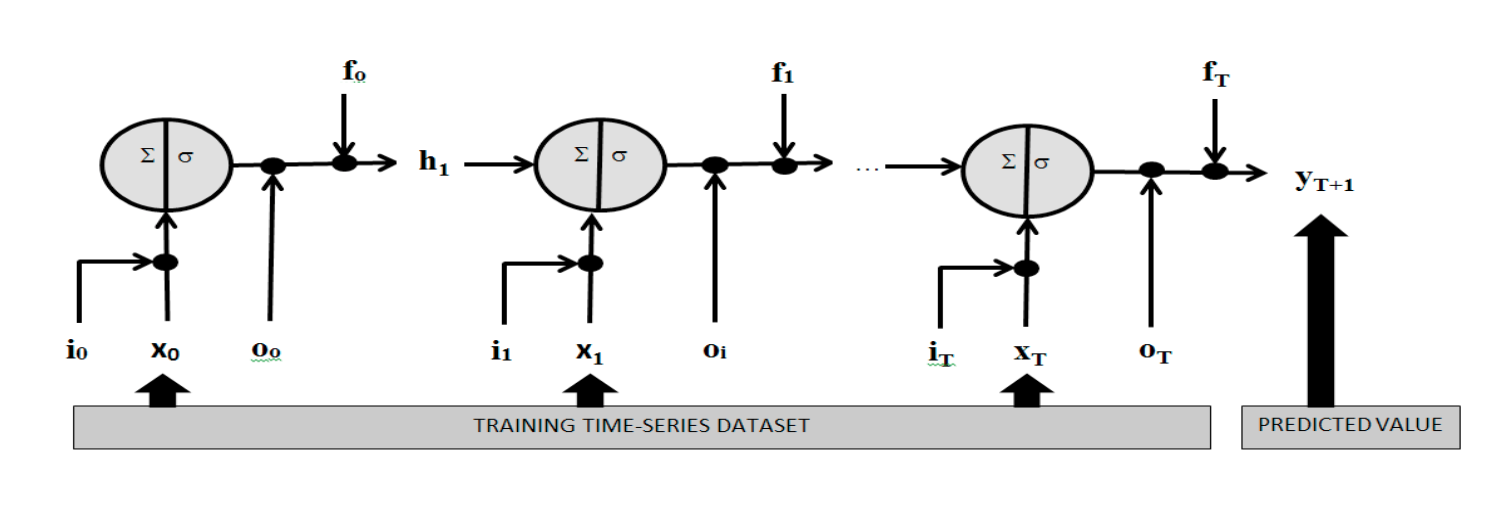
\includegraphics[width=1.0\linewidth]{images/LSTM.png}
    \caption{Architecture of Unfolded LSTM Model (\cite{salman2018single})}
    \label{fig:LSTM}
\end{figure}

\noindent As can be seen in Figure \ref{fig:LSTM} each LSTM block receives an input signal $x$, an input gate signal $i$, recurrent signal $h$, forget gate signal $f$ and produces an output gate signal $o$. LSTM networks compute a mapping of the input $(x_0,...,x_T)$ to an output sequence $(y_0,...,y_T)$ (\cite{salman2018single}). This is done by calculating the network unit activations using the following formulas (\cite{hochreiter1997long}). 

\begin{equation}
    i_t = \sigma(W_i x_t + U_i h_{t-1} + b_i)
    \label{eq:3}
\end{equation}

\begin{equation}
    z_t = \tanh(W_z x_t + U_z h_{t-1} + b_z)
    \label{eq:4}
\end{equation}

\begin{equation}
    f_t = \sigma(W_f x_t + U_f h_{t-1} + b_f)
    \label{eq:5}
\end{equation}

\begin{equation}
    C_t = i_t * z_t + f_t * C_{t-1}
    \label{eq:6}
\end{equation}

\begin{equation}
    o_t = \sigma(W_o x_t + U_o h_{t-1} + V_o C_t + b_o)
    \label{eq:7}
\end{equation}

\begin{equation}
    h_t = o_t * \tanh(C_t)
    \label{eq:8}
\end{equation}

\noindent Standard recurrent neural networks often suffer from the vanishing gradient problem, which is a disadvantage when learning over long sequences of data. LSTMs mitigate this issue by incorporating specialized gating mechanisms that preserve gradients over time (\cite{hochreiter1997long}). $W_i, U_i, W_z, U_z, W_f, U_f, W_o$ and $U_o$ are all model parameters which need to be estimated during training of the model with known data. While this model has some increase in computational time, the benefit of a more accurate model is in this case prioritized (\cite{salman2018single}). 

\vspace{0.25cm}

\noindent The memory cell, $C_t$, in combination with the input, forget, and output gates enables the LSTM to hold valuable information over long durations while discarding less relevant data. This design is key to its ability to capture long-term dependencies and adapt to rapid changes in weather conditions, making it suitable for forecasting in dynamic offshore environments.

\section{Comparative Analysis}
\label{lit:comparative}
Although historical models like NWP, SF and EF provide a good foundation for weather forecasting and give relatively accurate results, it is important to look at their shortcomings. For the usage in offshore wind turbine installation, it is important that the models can be easily adapted to fluctuating data. This is where these models are less efficient in terms of handling non-linear patterns, accuracy for long-term forecasts and localized forecasts. Offshore weather forecasting needs models which can predict dynamic and local conditions but also need to be able to adapt quickly to sudden changes (\cite{Zhang2019}).

\vspace{0.25cm}

\noindent From this follows the reason to investigate new applicable models. In the research, the focus will be on 3 different types of models. Firstly, a hybrid model consisting of the historical model ARIMA, for linear behaviour, and combining this with a new ANN, to capture non-linear behaviour. This model is highly suitable in environments where both smooth trends and abrupt changes occur. Research has shown that hybrid models can significantly improve forecast accuracy by combining the strengths of statistical and machine learning approaches (\cite{zhang2003time}, \cite{buyuksahin2019improving}). Secondly, a probabilistic model in the form of BNN. By incorporating Monte Carlo Dropout, the BNN efficiently approximates Bayesian inference, offering a predictive distribution that quantifies uncertainty-making in highly variable offshore conditions (\cite{gal2016dropout}, \cite{mae2022uncertainty}). Finally, a deep-learning model in the form of an LSTM. LSTM networks have proven effective in various forecasting applications due to their ability to model both short-term fluctuations and long-term dependencies in time series data (\cite{siami2019comparison}). All strengths and Limitations are shown in Table \ref{table:comparative_models}. 

\begin{table}[h!]
\centering
\caption{Comparative Analysis of Advanced Forecasting Models for Offshore Applications}
\label{table:comparative_models}
\begin{tabular}{|p{2cm}|p{6.3cm}|p{6cm}|}
\hline
\centering \textbf{Model} & \textbf{Strengths} & \textbf{Weaknesses} \\ \hline 
\vspace{5pt}
\centering\textbf{ARIMA-ANN} & 
Based on ARIMA's ability to capture linear trends\newline
Augmented by ANN's capacity for non-linear pattern recognition\newline
Effective when both linear and non-linear fluctuations are present
& 
Requires careful tuning to balance ARIMA and ANN components\newline
Performance depends on the quality of ARIMA residuals \\ \hline
\vspace{5pt}
\centering\textbf{BNN (with MCD)} &
Provides probabilistic forecasts with uncertainty quantification\newline
Facilitates risk assessment in dynamic offshore conditions
& 
Complex implementation and interpretation\newline
Higher computational overhead than deterministic models \\ \hline
\vspace{5pt}
\centering\textbf{LSTM} &
Excels at capturing long-term dependencies and complex dynamics\newline
Adept at modelling evolving non-linear time series data
& 
Requires large datasets and significant computational resources\newline
Maybe less interpretable compared to hybrid or probabilistic models \\ \hline
\end{tabular}
\end{table}

\noindent Since these comprehensive models demand more computation, their better accuracy and flexibility provide large benefits in forecasting the changing and localized conditions of offshore weather forecasting.

\section{Previous Research}
\label{lit:previous}
Earlier research has been done on the same subject by H. Boer and C. Overvliet, relevant findings, for this research, are included in this section.

\subsection{Research Boer}
The first research was done by H. Boer, the focus of this research was how the cost and installation time of offshore wind turbines are influenced by weather conditions. This was done with a numerical weather prediction, NWP, to simulate expected weather predictions and compare these with calm water situations. Key findings of this report are found in the influential met-ocean data on the installation face, these were significant wave height, wave frequency and wind speed. These parameters can have a maximum value, visible in Table \ref{table:operational_limits}, to ensure the installed ships can be used. 

\begin{table}[h!]
\centering
\caption{Operational Limits for Key Weather Conditions During Installation Phases}
\begin{tabular}{|l|c|c|c|c|c|c|}
\hline
\textbf{Phase} & \textbf{Vessel} & \textbf{Wave Height} & \textbf{Wave Frequency} & \textbf{Wind Speed} \\
\hline
\multirow{3}{*}{Monopile} & Crane Barge & 1.0 & 9 & 10 \\
 & HLV & 1.5 & 9 & 16 \\
 & Jack-Up & 2.5 & - & 16 \\
\hline
\multirow{3}{*}{Transition Piece} & Crane Barge & 1.0 & 9 & 10 \\
 & HLV & 1.5 & 9 & 16 \\
 & Jack-Up & 2.5 & - & 16 \\
\hline
\multirow{3}{*}{Tower} & Crane Barge & 1.0 & 7 & 10 \\
 & HLV & 1.5 & 7 & 10 \\
 & Jack-Up & 2.5 & - & 10 \\
\hline
\multirow{3}{*}{Nacelle} & Crane Barge & 1.0 & 7 & 10 \\
 & HLV & 1.5 & 7 & 10 \\
 & Jack-Up & 2.5 & - & 10 \\
\hline
\multirow{3}{*}{Blade} & Crane Barge & 1.0 & 7 & 8 \\
 & HLV & 1.5 & 7 & 8 \\
 & Jack-Up & 2.5 & - & 8 \\
\hline
\end{tabular}
\label{table:operational_limits}
\end{table}

\noindent Overall the report emphasizes how important accurate weather forecasting is in the installation phase of offshore wind turbines to minimize delays and so reduce costs. The simulated model underscores the importance of accurate weather forecasting, where this research compares calm weather with weather-restricted scenarios, it becomes clear why accurate weather forecasting is necessary (\cite{boer2022installation}).

\subsection{Research Overvliet}
The second research was conducted by C. Overvliet, this study focuses on quantifying the impact of increasing uncertainty in the weather forecasts on the delays and costs associated with the installation phase of offshore wind turbines. In this research, one specific location in the North Sea was used for data training, learning and testing. The models used are an Artificial Neural Network (ANN), an Auto-Regressive Integrated Moving Average (ARIMA), and a Long-Short Term Memory (LSTM). All these models are evaluated separately to determine their effectiveness in predicting weather conditions. 
\\

\noindent Where ARIMA models only showed the linear trends, it was chosen to further investigate the non-linear behaviours in the data. With high variability in the weather, such as sudden changes in wind speed and wave height, it showed the ANN and LSTM models made more accurate forecasts. ANN provided a model which identifies the non-linear relationship between the different influential variables. While LSTM offered an extra advantage in capturing long-term dependencies in the met-ocean data. 
\\

\noindent Another key finding in the report shows the relationship between the forecast accuracy and how this directly impacts the scheduling and associated costs of the installation phase. The greater the uncertainty, the higher the operational costs that follow from delays due to weather constraints. Overall it shows the importance of reducing the accuracy and so having a smoother and more efficient operation (\cite{overvliet2023uncertainty}).